\section{Projektmanagement}

\subsection{Projektübersicht}
Das Hauptziel dieser Studienarbeit ist die Installation von DNA-Center und Integration vom bestehenden Labor-Netzwerk.

\subsubsection{Ziele der Projektes}
Da Software-Defined Access Neuland im Campus Bereich ist, wollen wir die SD-Access Lösung vom Hersteller Cisco ausarbeiten. Dazu gehören folgende Ziele:

\begin{itemize}
	\item Installation von DNA-Center und Integration vom bestehenden Campus Labor-Netzwerk.
	\item Definieren von Benutzer- und Geräteprofilen, um basierend auf Geschäftsanforderungen die Zugriffsrechte und Netzwerksegmentierung zu veralten und so das Netzwerk sicher zu halten.
	\item Verwendung von Erkenntnissen von DNA Analytics and Assurance für eine proaktive Überwachung, Fehlerbehebung und Optimierung des Netzwerks.
	\item Integration vom bestehenden IP Address Management Tool im DNA Center
	\item Durch APIs, Erstellung von wöchentlichen Reports über den Campus Netzwerk Status in einem E-Mail und einer Slack Message. 
\end{itemize}

\subsection{Projektorganisation}
Diese Studienarbeit wird von drei Personen umgesetzt und durch zwei Betreuer überwacht.

\subsubsection{Organisationsstruktur}
\begin{figure}[H]
	\centering
	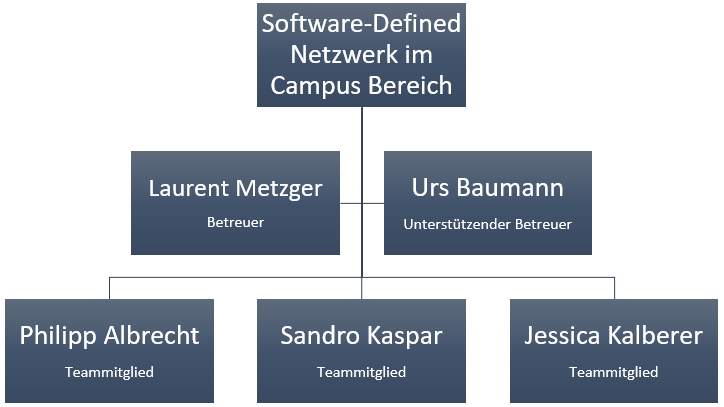
\includegraphics[height=5cm]{img/Organisationsstruktur.png}
	\caption{Organisationsstruktur}
	\label{fig:Organisationsstruktur}
\end{figure}

\subsection{Management Abläufe}
Für die Umsetzung der Studienarbeit stehen insgesamt 15 Wochen und pro Person 240 Stunden zur Verfügung. In einer Woche liegt das Arbeitspensum von 16 Stunden pro Person vor. Das Projekt startet am 19. Februar 2018 und endet am 1. Juni 2018.

\subsubsection{Zeitliche Planung}
Die zeitliche Planung erfolgte in Gant und die Verwaltung der Arbeitspakete auf Waffle.io. Die Planung wird während dem Projekt laufend aktualisiert und angepasst. Die Zeiterfassung erfolgt während der Arbeitsausführung mit Toggle getrackt.

\begin{figure}[H]
	\centering
	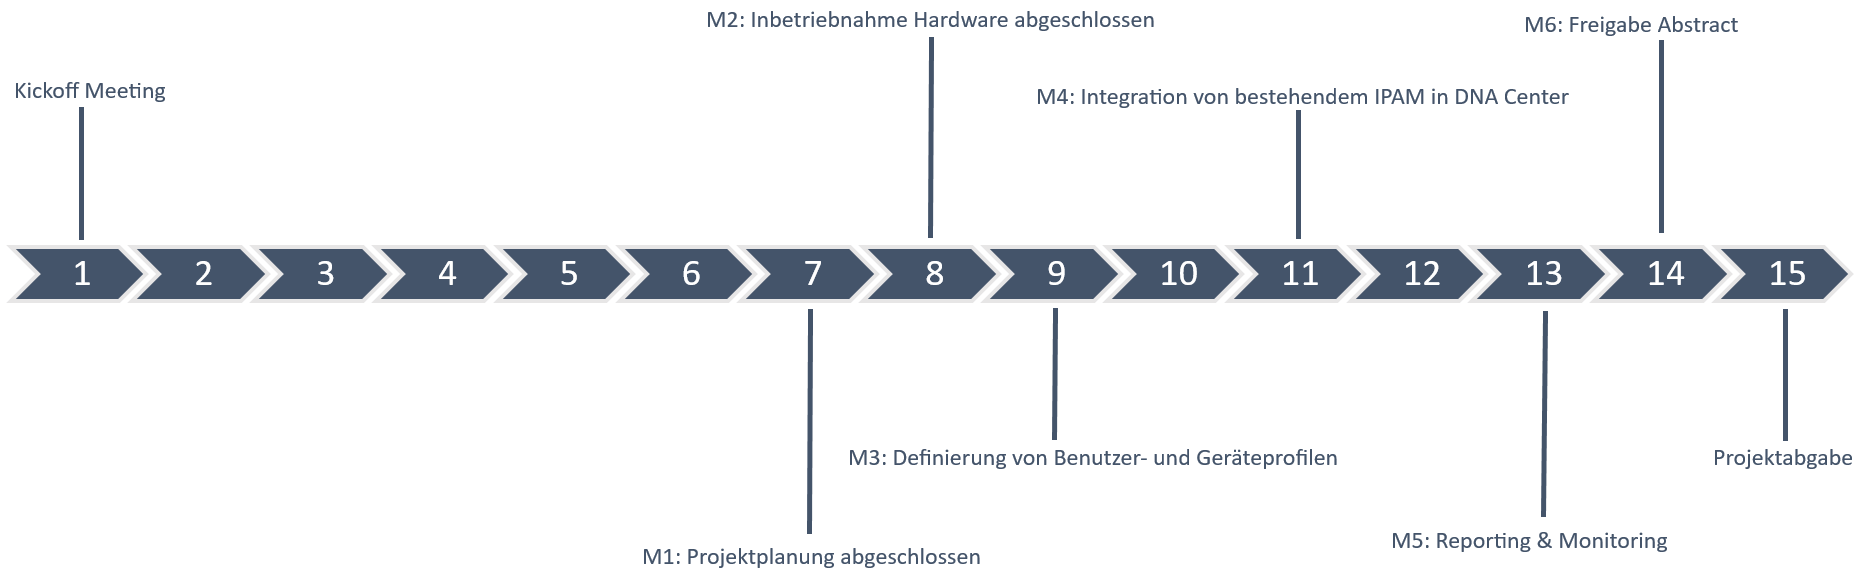
\includegraphics[height=5cm]{img/ZeitlichePlanung_v3.png}
	\caption{Projektplanung}
	\label{fig:Projektplanung}
\end{figure} 

\subsubsection{Meilensteine}
Folgende Meilensteine sind für das Projekt definiert:
\begin{table}[H]
	\rowcolors{2}{gray!25}{white}
	\centering
	\begin{tabularx}{\textwidth}{p{1cm}| p{2.5cm}| X}
		\rowcolor{gray!50}
		\textbf{Nr} & \textbf{Datum} & \textbf{Meilenstein} \\
		\hline	
		M0 & 27.02.2018 & Kickoff Meeting \\
		M1 & 20.03.2018 & Projektplanung abgeschlossen \\
		M2 & 10.04.2018 & Inbetriebnahme Hardware abgeschlossen \\
		M3 & 17.04.2018 & Definierung von Benutzer- und Geräteprofilen \\
		M4 & 01.05.2018 & Integration von bestehenden IPAM in DNA Center \\
		M5 & 15.05.2018 & Reporting \& Monitoring \\
		M6 & 28.05.2018 & Freigabe des Abstracts \\
		M7 & 01.06.2018 & Abgabe Projekt \\
	\end{tabularx}
	\caption{Meilensteine}
	\label{tab:Meilensteine}
\end{table}

\subsubsection{Arbeitspakete}
Alle Arbeitspakete werden in Waffle.io erfasst und sind unter folgendem Link ersichtlich:
\href{Waffle.io}{https://waffle.io/night28/HSR\_SA}
\subsubsection{Besprechungen}
Die Besprechungen mit dem Betreuer finden an den nachfolgend aufgelisteten Tagen statt:
\begin{itemize}
	\item jeden Dienstag zwischen 15.10 - 16.10 Uhr
\end{itemize}

Offene Traktanden und Probleme werden mit dem Betreuer kommuniziert und diskutiert. Nach dieser Besprechung wird jeweils in einem Team-Meeting das weitere Vorgehen geplant.


\subsection{Infrastruktur}
Die Organisation der Arbeit und Teammitglieder wird durch folgende Werkzeuge unterstützt:

\begin{figure}[H]
	\centering
	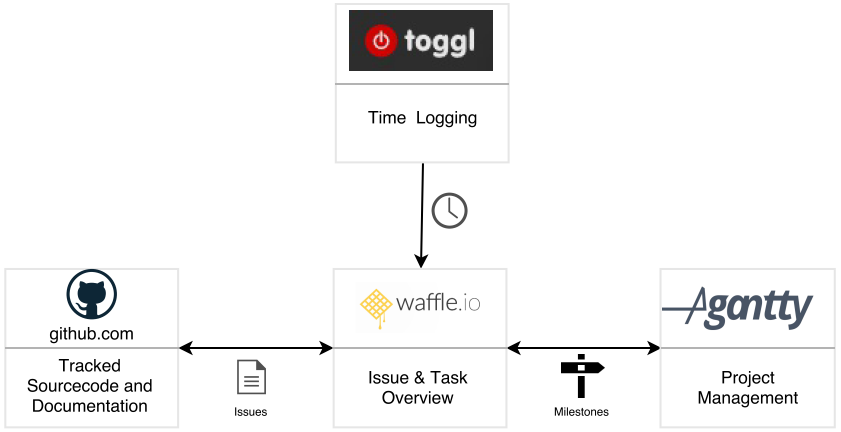
\includegraphics[height=6cm]{img/InterneOrganisationsstruktur.png}
	\caption{Interne Organisationsstruktur}
	\label{fig:Interne Organisationsstruktur}
\end{figure} 

Unsere Tools sind unter folgenden Links ersichtlich:
\paragraph{GitHub} \href{https://github.com/night28/HSR_SA}{https://github.com/night28/HSR\_SA} 

\paragraph{Waffle.io} \href{https://waffle.io/night28/HSR\_SA}{https://waffle.io/night28/HSR\_SA}

\paragraph{Toggl} \href{https://toggl.com/}{https://toggl.com/}

\paragraph{Agantty} \href{https://app.agantty.com/\#/project/203670}{https://app.agantty.com/\#/project/203670}
 
\subsection{Risiko Management}

\subsubsection{Umgang mit Risiken}

Risiken lassen sich leider nicht immer vermeiden. Aus diesem Grund sind nachfolgend mögliche Risiken aufgeführt. Des Weiteren wurden vorbeugende Massnahmen definiert, um die Eintrittswahrscheinlichkeit von Risiken mit schwerwiegenden Konsequenzen zu reduzieren. Für den Fall, dass ein Risiko dennoch eintreten sollte, sind entsprechende Massnahmen definiert um den Schaden möglichst gering zu halten.
Sollten sich während dem Projekt neue potenzielle Risiken zeigen, wird dieses Dokument laufend aktualisiert.

\begin{landscape}

\subsubsection{Risiken}
\newcommand*\rot{\rotatebox{90}}
\begin{longtable}{|m{0.5cm}|m{3cm}|m{5cm}|m{0.75cm}|m{0.75cm}|m{0.75cm}|m{5cm}|m{5cm}|} 
	\hline
	\rot{Nummer} & \rot{Titel} & \rot{Beschreibung} & \rot{\shortstack[l]{maximaler\\Schaden [h]}} & \rot{\shortstack[l]{Eintritts-\\wahrscheinlichkeit}} & \rot{\shortstack[l]{Gewichteter\\Schaden [h]}} & \rot{Vorbeugung} & \rot{\shortstack[l]{Verhalten beim\\Eintreten}} \\
	\hline\hline
	1 & Ausfall eines Teammitglieds & Ausfall auf Grund unvorhergesehener Ereignisse wie Krankheit, Unfall etc. & 40 & 15\% & 6 & Reserven einplanen, Kommunikation sicherstellen, damit andere Teammitglieder die Aufgaben übernehmen können & Tasks des ausgefallen Mitglieds möglichst auf die anderen Teammitglieder aufteilen. \\ 
	\hline
	2 & Hardwareausfall DNA-Center & DNA-Center Appliance fällt durch Hardwaredefekt aus & 30 & 5\% & 1.5 & keine Verbeugenden Massnahmen möglich & Austausch im Rahmen der Garantie veranlassen \\
	\hline
	3 & Fehlendes Know-How & Da viele der Themen neu sind, kann entsprechendes Wissen fehlen & 40 & 20\% & 8 & Zeit einplanen um sich in neue Themen einzuarbeiten & Fehlendes Wissen sobald wie möglich aneignen. Bei Bedarf Rat der Betreuer einholen \\
	\hline
	4 & Konflikte oder Missverständnisse im Team & Das Team ist sich bezüglich wichtigen Entscheidungen uneinig & 25 & 15\% & 3.75 & Entscheidungen stets mit Begründung dokumentieren & Kann auch mit Hilfe der Doku keine Einigung gefunden werden, fachnlichen Rat des Betreuers einholen \\
	\hline
	5 & Missverständnisse im Team & Im Team herscht Uneinigkeit über bereits getroffene Entscheidungen & 20 & 20\% & 4 & Protokolle führen und Entscheidungen klar dokumentieren & Protokolle und Dokumentationen beiziehen \\
	\hline
	6 & Ausfall Server / Netzwerkinfrastruktur & Ausfall der von der HSR zur Verfügung gestellten Infrastrukturkomponenten & 30 & 10\% & 3 & Keine Vorbeugenden Massnahmen möglich & Sobald die Infrastruktur wieder verfügbar ist, Systeme erneut in Betrieb nehmen \\
	\hline
	7 & Lieferverzögerung Hardware & Die von Cisco bestellte Hardware kommt später als angekündigt & 30 & 18\% & 5.4 & Keine Vorbeugenden Massnahmen möglich & Projektplanung an neue Gegebenheiten anpassen, notfalls Projektumfang in Absprache mit Betreuer anpassen \\
	\hline
	8 & Zeitaufwände falsch geschätzt & Auf Grund falscher Schätzungen kommt es zu Verzögerungen im Projekt & 30 & 25\% & 7.5 & Laufende Kontrolle des Projektfortschritts um Probleme frühzeitig zu erkennen, Reserven einplanen & Verbleibende Schätzungen korrigieren, Planung anpassen \\
	\hline
	9 & Datenverlust & Verlust von projektbezogenen Daten wie Dokumentationen, Konfigurationen etc. & 40 & 5\% & 2 & Regelmässige und verteilte Backups aller Daten erstellen & Verlorenen Daten aus Backups wiederherstellen, fehlende Daten neu erarbeiten \\
	\hline
	10 & Unausgereifte Software & Verzögerung des Projektes durch unvorhergesehene Hürden, da Software nicht genügend auf Funktionalität getestet und Dokumentiert. Software steht noch in einem frühen Release. & 80 & 5\% & 4 & Über aktuelle Funktionalitäten und Bugs informieren & Bugs reporten und bei Möglichkeit diese umgehen. Falls nötig Hilfe beim Hersteller suchen. \\
	\hline
\end{longtable}

\end{landscape}

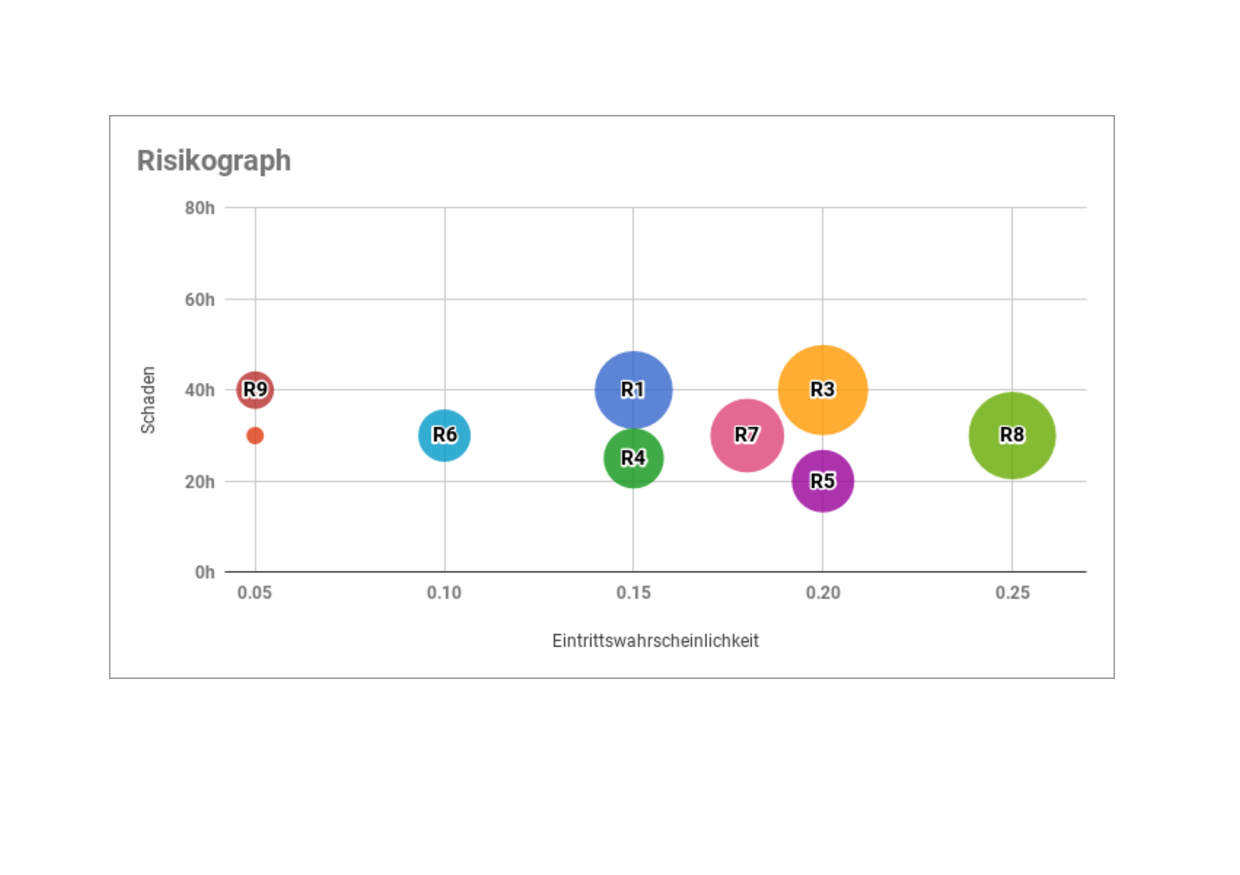
\includepdf{pdfincludes/risikograph}

\subsubsection{Eingetretene Risiken}
Nachfolgend werden die eingetretenen Risiken genauer erläutert.
\paragraph{Lieferverzögerung Hardware}
Leider wurde die Hardware nicht wie geplant geliefert. Deshalb wurde die Projektplanung an die neuen Gegebenheiten angepasst. \\
Nachfolgend die alte Projektplanung:
\begin{figure}[H]
	\centering
	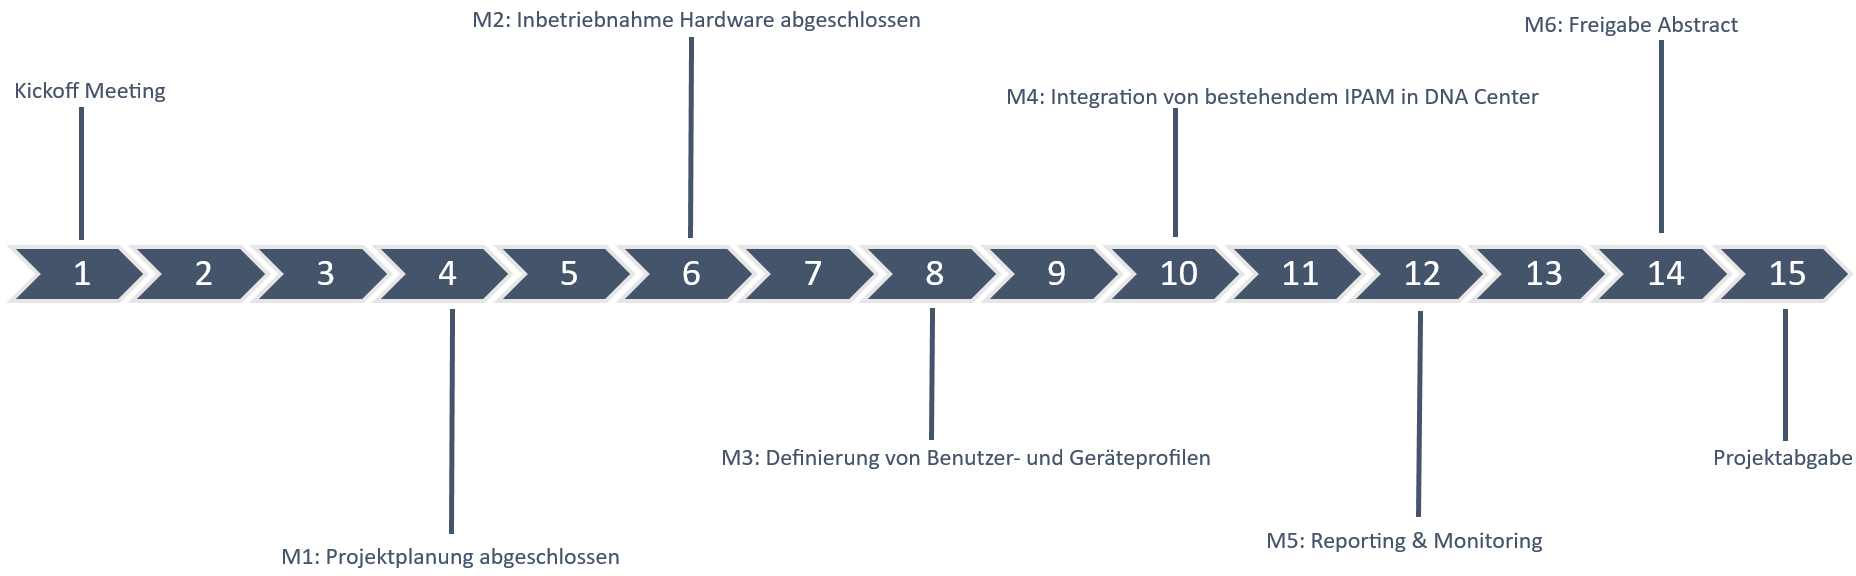
\includegraphics[height=5cm]{img/ZeitlichePlanung_v1.png}
	\caption{alte Projektplanung}
	\label{fig:alte Projektplanung}
\end{figure} 

Folgende Meilensteine waren für das Projekt definiert:
\begin{table}[H]
	\rowcolors{2}{gray!25}{white}
	\centering
	\begin{tabularx}{\textwidth}{p{1cm}| p{2.5cm}| X}
		\rowcolor{gray!50}
		\textbf{Nr} & \textbf{Datum} & \textbf{Meilenstein} \\
		\hline	
		M0 & 27.02.2018 & Kickoff Meeting \\
		M1 & 20.03.2018 & Projektplanung abgeschlossen \\
		M2 & 03.04.2018 & Inbetriebnahme Hardware abgeschlossen \\
		M3 & 17.04.2018 & Definierung von Benutzer- und Geräteprofilen \\
		M4 & 01.05.2018 & Integration von bestehenden IPAM in DNA Center \\
		M5 & 15.05.2018 & Reporting \& Monitoring \\
		M6 & 28.05.2018 & Freigabe des Abstracts \\
		M7 & 01.06.2018 & Abgabe Projekt \\
	\end{tabularx}
	\caption{alte Meilensteine}
	\label{tab:alte Meilensteine}
\end{table}

Die neue Projektplanung sieht nun folgendermassen aus:
Nachfolgend die alte Projektplanung:
\begin{figure}[H]
	\centering
	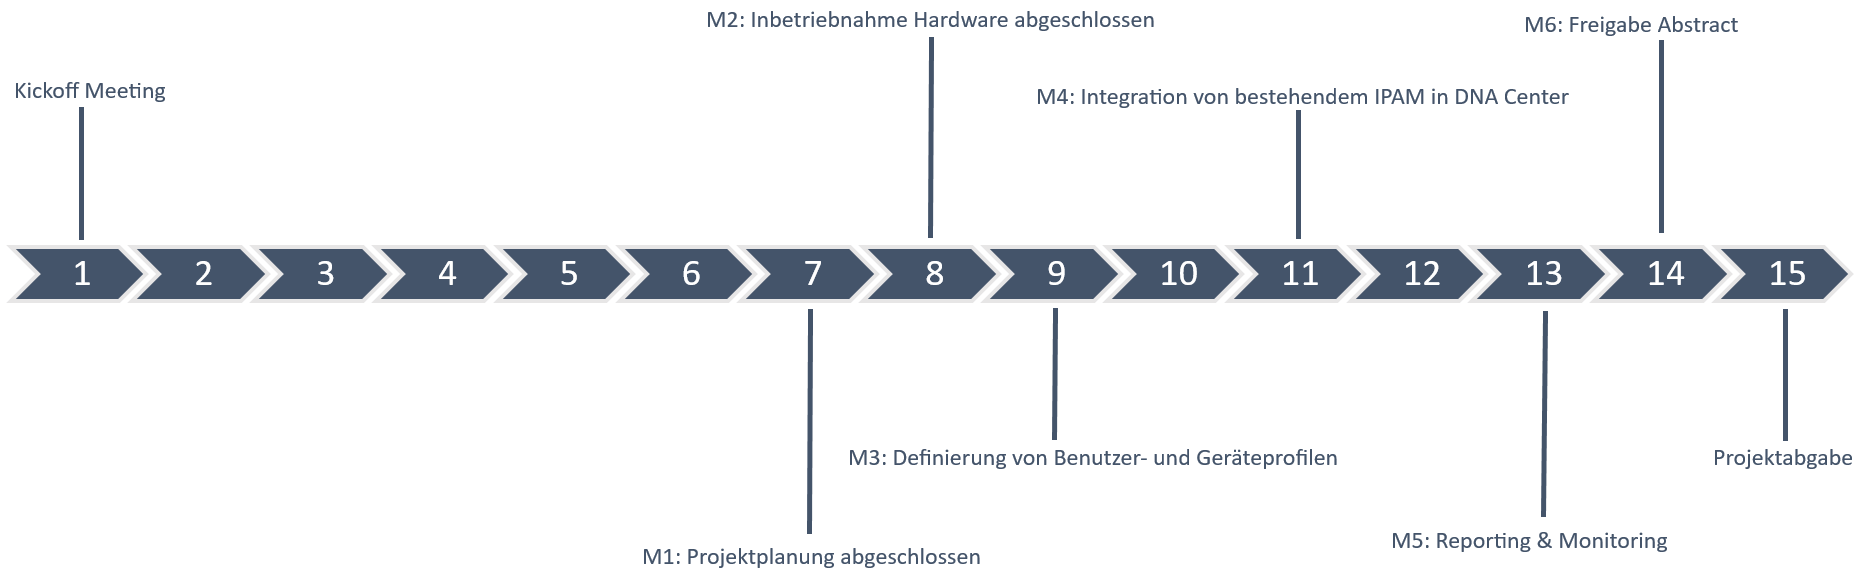
\includegraphics[height=5cm]{img/ZeitlichePlanung_v3.png}
	\caption{neue Projektplanung}
	\label{fig:neue Projektplanung}
\end{figure} 


Folgende Meilensteine sind nun aufgrund der Lieferverzögerung für das Projekt definiert:
\begin{table}[H]
	\rowcolors{2}{gray!25}{white}
	\centering
	\begin{tabularx}{\textwidth}{p{1cm}| p{2.5cm}| X}
		\rowcolor{gray!50}
		\textbf{Nr} & \textbf{Datum} & \textbf{Meilenstein} \\
		\hline	
		M0 & 27.02.2018 & Kickoff Meeting \\
		M1 & 10.04.2018 & Projektplanung abgeschlossen \\
		M2 & 17.04.2018 & Inbetriebnahme Hardware abgeschlossen \\
		M3 & 24.04.2018 & Definierung von Benutzer- und Geräteprofilen \\
		M4 & 08.05.2018 & Integration von bestehenden IPAM in DNA Center \\
		M5 & 22.05.2018 & Reporting \& Monitoring \\
		M6 & 28.05.2018 & Freigabe des Abstracts \\
		M7 & 01.06.2018 & Abgabe Projekt \\
	\end{tabularx}
	\caption{neue Meilensteine}
	\label{tab:neue Meilensteine}
\end{table}

\paragraph{Unausgereifte Software und fehlendes Know-How}
Das DNA Center befand sich beim Beginn unserer Studienarbeit noch in der Version 1.1.3. Bis zur Abgabe wurde die Version 1.1.6 veröffentlicht, auf welche wir unser DNA Center auch aktualisiert hatten. 
\begin{figure}[H]
	\centering
	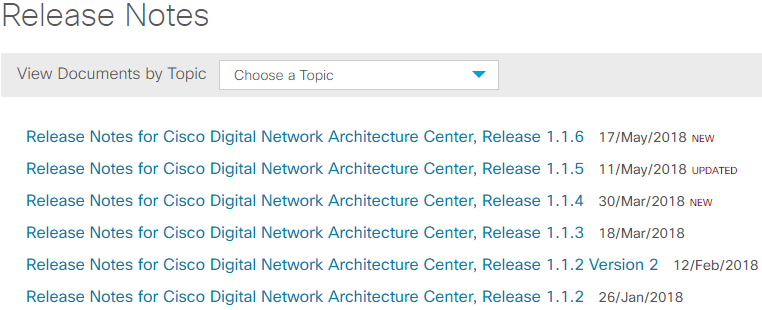
\includegraphics[height=6cm]{img/ReleaseNotes.png}
	\caption{Release Notes}
	\label{fig:Release Notes}
\end{figure}
Das DNA Center enthält in diesen frühen Versionen noch viele Bugs und auch Beta Features, welche oft zu Problemen führen können. Die Funktionalitäten sind teilweise nur beschränkt so umsetzbar, wie sie angekündigt und beschrieben wurden. 
Bei unserem ersten Versuch mit der Version 1.1.3 stiessen wir auf das Problem, dass wir die Geräte über die LAN Automation nicht durchführen konnten, da nicht einmal ein DHCP Server auf den Geräten konfiguriert wurden. Weitere Probleme kamen auch beim Provisionierungsprozess hinzu. Geräte welche vorher verwaltet werden konnte, waren auf einmal nicht mehr erreichbar im DNA Center, obwohl dies manuell per SSH kein Problem darstellte. Ein Versuch das DNA Center per Backup zu sichern, brachte das ganze DNA Center zum Absturz. Nachdem viele solche Hürden und Probleme aufgetaucht waren, entschieden wir uns es mit einem Out of Band Management zu versuchen. Hierzu musste der Konfigurations-Wizard des DNA Centers nochmal gestartet werden, um das zweite Netzwerkinterface zu definieren. Das erneute Durchführen dieses Konfigurations-Wizard führte zum kompletten Absturz, so dass die ganze DNA Center Appliance gar nicht mehr bootete. \\
Nach einer zweiten Installation des DNA Centers versuchten wir erneut die LAN Automation, um ein Underlay zu bereitzustellen. Diesmal funktionierte das Hinzufügen eines Seed-Devices. Die LAN Automation soll nach der Konfiguration eines Seed-Devices so oft wie nötig gestartet und gestoppt werden können. Sollte später ein weiterer Switch hinzu kommen, so könnte diese erneut für dieses Device gestartet werden. In unserem Fall führe dies zu Problemen mit der Konfiguration des IS-IS Protokolls. Es wurden nur die Routen der ersten Geräte zum Border hinzugefügt. Die Routen aller nachfolgenden Geräte wurden nur beliebig oder gar nicht hinzugefügt, so dass diese keine Kommunikation zum DNA Center aufbauen konnten. 
Dies führte bei einigen Konfiguration zur Verwirrung, da wir teilweise nicht wussten ob es sich um ein falsches Verhalten der Software oder einen Fehler unsererseits handelte. Aus diesem Grunde wurde beschlossen uns für einen Tag einen Cisco Experten zur Verfügung zu stellen. Wir konnten mit ihm die Konfiguration nochmal von Grund auf durchführen und kamen bis zur Konfiguration eines Seed-Devices für die LAN Automation. An diesem Punkt stiessen wir aber wieder auf diverse Hindernisse, bei welchen uns der Cisco Experte zu dieser Zeit nicht weiterhelfen konnte. Nach eigenen weiteren Versüchen gelang es uns jedoch, die LAN Automation auf einem weiteren Gerät durchzuführen.\\
Des Weiteren Fehlen Dokumentationen zu der Verwendung von Policies oder der genauen Verwendung der Authentication Templates für das Onboarding. Bei dieser Bedeutung der verschiedenen Authentication Templates konnte uns jedoch jemand von Cisco Auskunft geben. 

Da bei uns bereits zwei eher schwerwiegende Risiken eingetreten waren, wurde entschieden das der Abgabetermin um knapp zwei Wochen, auf den 13. Juni 2018 verschoben wird. Das hat folgende Anpassungen in der Projektplanung zur Folge:


\begin{figure}[H]
	\centering
	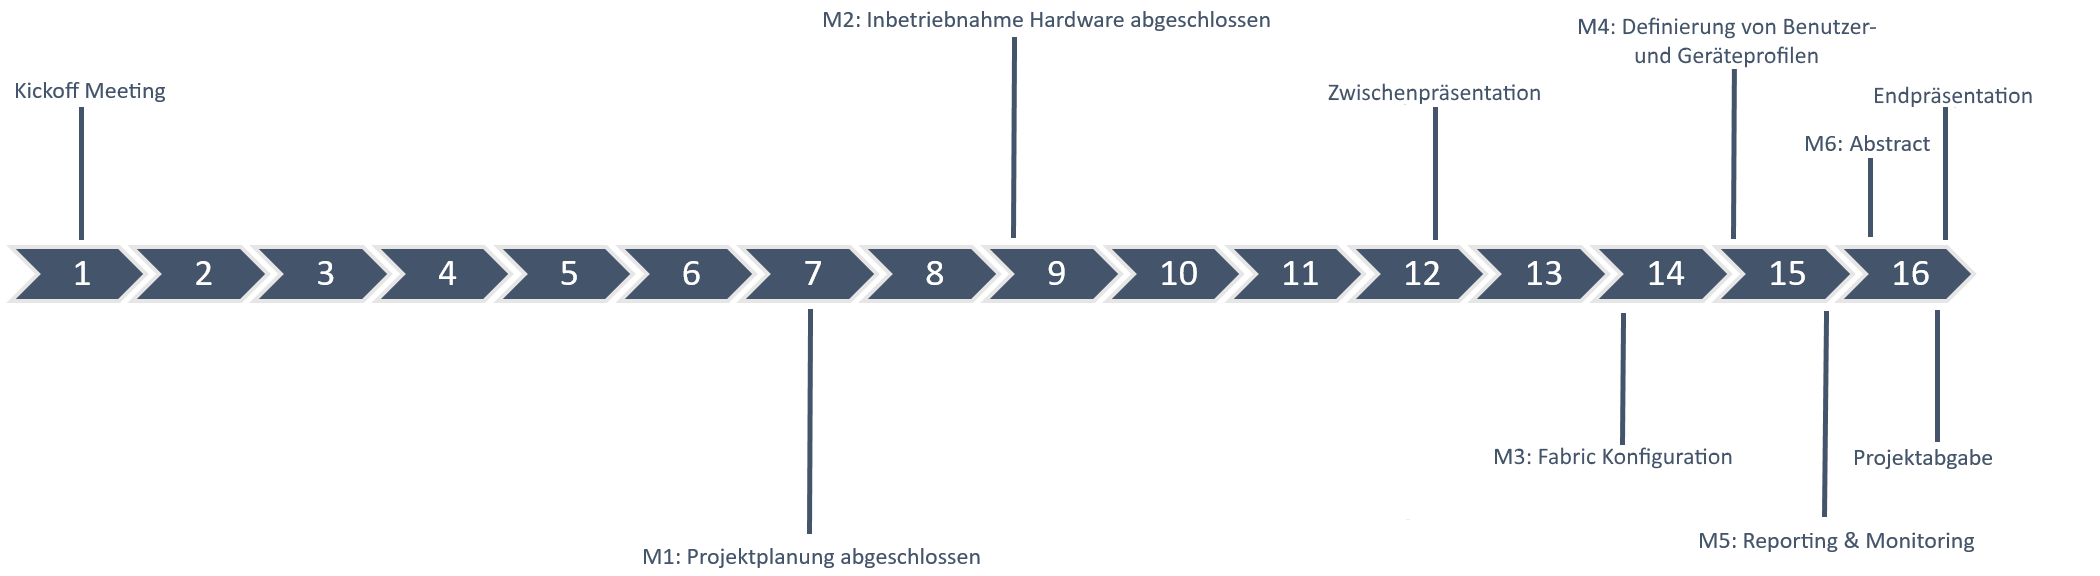
\includegraphics[width=16cm]{img/ZeitlichePlanung_v4.png}
	\caption{Erweiterte Anpassung der Projektplanung}
	\label{fig:Erweiterte Anpassungen der Projektplanung}
\end{figure} 


Folgende Meilensteine sind nun aufgrund der Lieferverzögerung für das Projekt definiert:
\begin{table}[H]
	\rowcolors{2}{gray!25}{white}
	\centering
	\begin{tabularx}{\textwidth}{p{1cm}| p{2.5cm}| X}
		\rowcolor{gray!50}
		\textbf{Nr} & \textbf{Datum} & \textbf{Meilenstein} \\
		\hline	
		M0 & 27.02.2018 & Kickoff Meeting \\
		M1 & 10.04.2018 & Projektplanung abgeschlossen \\
		M2 & 24.04.2018 & Inbetriebnahme Hardware abgeschlossen \\
		   & 16.05.2018 & Zwischenpräsentation \\
		M3 & 01.06.2018 & Fabric Konfiguration \\
		M4 & 10.06.2018 & Definierung von Benutzer- und Geräteprofilen \\
		M5 & 12.06.2018 & Reporting \& Monitoring \\
		M6 & 13.06.2018 & Freigabe des Abstracts \\
		M7 & 13.06.2018 & Abgabe Projekt \\
		   & 15.06.2018 & Endpräsentation \\
	\end{tabularx}
	\caption{Erweiterte Anpassung der Meilensteine}
	\label{tab:Erweiterte Anpassung der Meilensteine}
\end{table}

Auf der Grafik ist ersichtlich, dass die komplette Konfiguration des DNA Centers nach der Zwischenpräsentation stattfindet. Geplant war die Fabric Konfiguration schon in der zehnten Woche, jedoch funktionierte zu diesem Zeit die LAN Automation nur mässig und die Geräte wurden manuell zum DNA Center hinzugefügt, so dass eine Fabric konfiguriert werden konnte. Kurz vor der Zwischenpräsentation war die Definierung der Benutzer- und Geräteprofilen wichtig, da an der Präsentation unter anderem die Konnektivität zwischen zwei Clients vorgeführt werden sollte. Dies war jedoch wegen mehreren aufgetretenen Fehlern und Problemen nicht möglich. Der Versuch das DNA Center nochmals von vorne zu mit einem Out of Band Management zu Konfigurieren scheiterte leider. Der Maglev Configuration Wizard brach am Schluss der Konfigurationen mit einem Fehler ab und brachte das ganze DNA Center in einen "not bootable" Zustand. \\
Dies war ein guter Zeitpunkt um die komplette Installation des DNA Center nochmal sauber von vorne zu beginnen. Durch die vielen aufgetretenen Probleme wurde uns wie schon oben erwähnt für einen Tag ein Cisco Experte zur Seite gestellt, mit welchen wir die Konfiguration des Underlay Netzwerkes bis zum Definieren eines ersten Seed-Devices durchführen konnten.




